\begin{figure}[!ht]
	\centering
	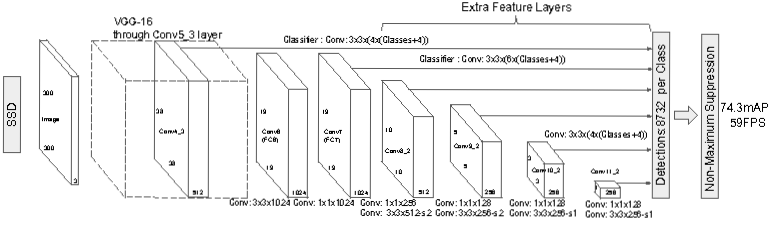
\includegraphics[width=0.8\textwidth]{chapter2/images/vgg.jpg}
		\caption{โครงสร้างทั่วไปของโมเดลปัญญาประดิษฐ์ SSD}
    	\label{fig:ssd}
\end{figure}

SSD เป็นโมเดลปัญญาประดิษฐ์ที่ใช้โครงข่ายประสาทเทียมตัวเดียวสำหรับการตรวจจับวัตถุ ซึ่งภายในโครงข่ายจะประกอบไปด้วยการทำงานหลัก 3 อย่าง คือ
\begin{enumerate}
	\setlength\itemsep{-0.25em}
	\item การสกัดคุณลักษณะ
	\\	นำรูปภาพทั้งรูปภาพเข้าผ่านVGG-16(เป็นโมเดล CNN ชนิดหนึ่ง) เพื่อการสกัดคุณลักษณะของรูปภาพ
	\item การทำนายผล
	\\	หลังจากที่ได้คุณลักษณะมาแล้วจะนำไปทำนายผลผ่าน Fully connected
	\item การเลือกคัดกรองผลลัพธ์
	\\	หลังจากได้ผลลัพธ์เป็นหมวดหมู่ของกรอบสี่เหลี่ยม และ ตำแหน่งของกรอบสี่เหลี่ยมจะนำไปผ่านกระบวนการ NMS เพื่อให้ได้ผลลัพธ์ที่ดีที่สุด  
\end{enumerate}

